\lesson{Wave Mechanics and Orbitals}
\begin{bulleted-list}
    \item Broglie hypothesized that if a wave can behave like a particle, then a particle should
        also be able to behave like a wave. His hypothesis was that electrons behaved like a wave
    \item According to Schrodinger, the electron can only have certain quantized energies because
        of the requirement for only whole numbers of wavelengths for the electron wave
\end{bulleted-list}

\subsection{Electron Orbitals}
\begin{bulleted-list}
    \item Heisenberg realized that to measure any particle, we essentially had to ``touch''
        it. The only way to do this is to shoot a photon at the electron and measure the
        photon. However, the process of hitting  a subatomic particle with a photon means that
        the particle is no longer where it was and it has also changed it speed. This is 
        \textbf{Heisenberg's uncertainty principle}
        \footnote{
            \textbf{Heisenberg's uncertainty principle:} it is impossible to know simultaneously
            the position and velocity of an electron.
        }
    \item Since the position of an electron is described as a region of probability, scientists
        use the term \textbf{orbital} to describe the region in space where electrons may be 
        found. See Figure \ref{fig:orbital-shapes}
\end{bulleted-list}

\begin{figure}[ht!]
    \centering
    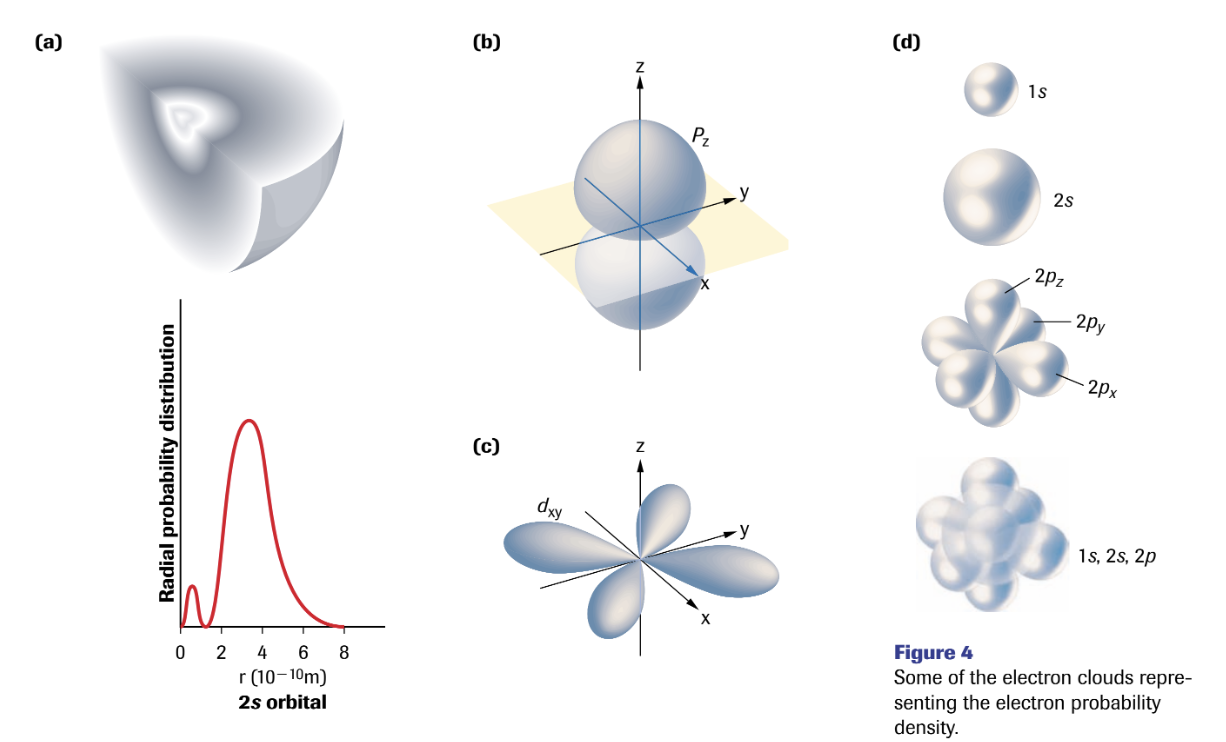
\includegraphics[width=0.8 \textwidth]{../figures/orbital-shapes.png}
    \caption{(a): In the cross-section, the darker theshading, the higher the \textbf{electron
    probability density}. (b): A $2p_z$ orbital. (c): A $d_{xy}$ orbital. (d): A 
    superposition of a 1s, 2s, and 2p orbitals.
}
    \label{fig:orbital-shapes}
\end{figure}

\begin{problems}
    \item Briefly state the main contribution of each of the following scientists to the 
        development of quantum mechanics:
        \begin{enum-alph}
            \item de Broglie
            \item Schrodinger
            \item Heisenberg
        \end{enum-alph}
    \item What is an electron orbital and how is it different from an orbit?
    \item State two general characteristics of any orbital provided by the quantum mechanics atomic
        model
    \item What information about an electron is not provided by the quantum mechanics atomic
        model?
    \item Using diagrams and words, describe the shapes of the 1s, 2s, and three 2p orbitals
    \item Theoretically, what is the maximum number of electrons in an atom that could have the
        following sets of quantum numbers
        \begin{enum-alph}
            \item $n=4$
            \item $n=5$, $m_\ell=+1$
            \item $n=5$, $m_s=+\frac{1}{2}$
            \item $n=3$, $\ell=2$
            \item $n=2$, $\ell=1$
            \item $n=0$, $\ell=0$, $m_\ell=0$
            \item $n=2$, $\ell=1$, $m_\ell=-1$, $m_s=-\frac{1}{2}$
            \item $n=3$
            \item $n=2$, $\ell=2$
            \item $n=1$, $\ell=0$, $m_\ell=0$
        \end{enum-alph}
    \item Using the Peridic Table, list elements (you may ignore the lathanides and actinides)
        that have ground state electron configurations that differ from those we would predict
    \item The electron configurations are determined experimentally for atoms in the gas phase.
        Would you expect the electron configurations to be the same in the solid and liquid
        states as in the gas phase?
\end{problems}

\begin{solutions}
    \item 
    \begin{enum-alph}
        \item de Broglie theorized that if a wave can behave like a particle, then a particle
            should also behave like a wave. His hypothesis was that an electron behaved like a
            wave
        \item Schrodinger theorized that electrons can only have certain quantized energies because
            of the requirement for only whole number wavelengths for the electron wave
        \item Heisenberg created the uncertainty principle which states that we cannot simultaneously
            know both the position and velocity of an electron
    \end{enum-alph}

    \item Bohr's and Rutherford's model both included electrons orbiting around the nucleus. An orbital
    on the other hand, is a electron probability dense region where electrons have a probability
    of appearing.
    \item The energy level that it is in and the shape.
    \item Position and velocity, according to Heisenberg's uncertainty principle
    \item The 1s orbital is a sphere that is not as dense in the center. The 2s orbital looks
        the same as the 1s orbital but larger. The three 2p orbitals look like dumbbells stacked
        perpendicular on top of each other
    \item 
        \begin{enum-alph}
            \item $e=2(4^2)=32$
            \item $e=\frac{1}{2}(2)(5^2)=25$
            \item $e=2(5)=10$
            \item $e=2(3)=6$
            \item $e=2$
            \item $e=1$
            \item $e=2(3^2)=18$
            \item $e=2(3)=6$
            \item $e=2$
        \end{enum-alph}
    \item The transition metals because they have d orbitals and can hybridize orbitals
    \item The electron configurations can differ in solid and liquid states compared to the gas
        states. This is because in solid and liquid states, the atoms are more closely packed,
        leading to interactions between neighbouring atoms
\end{solutions}
